\documentclass[10pt]{article}

%\usepackage{hyperref}
\usepackage{alltt}
\usepackage{natbib}
\usepackage{graphicx}
\usepackage{url}
\usepackage{fancyhdr}
\pagestyle{fancy}
\usepackage{trust-spi}
\usepackage{subfigure}
\usepackage{ifthen}
\usepackage{amsmath}
\usepackage{stmaryrd}

\usepackage{tikz}
\usetikzlibrary{arrows,shadows,matrix}
\usepackage[underline=false]{pgf-umlsd}

\lhead{ArmoredSoftware Architecture}
\rhead{Alexander, Gill, Kulkarni, Searl}
\lfoot{\copyright The University of Kansas, 2013}
\cfoot{\thepage}


\newboolean{submission}  %%set to true for the submission version
\setboolean{submission}{false}
%\setboolean{submission}{true}
\ifthenelse
{\boolean{submission}}
{ \newcommand{\todo}[1]{ } } % hide todo
{ \newcommand{\todo}[1]{ % show todo
   \marginpar{\raggedright\footnotesize{#1}}
               }}
\newcommand{\squash}{\parskip=0pt\itemsep=0pt}

\parskip=\medskipamount
\parindent=0pt


\bibliographystyle{abbrvnat}

\title{ArmoredSoftware Semantics 0.0}
\author{ArmoredSoftware Crew \\
Information and Telecommunication Technology Center \\
The University of Kansas \\
\url{palexand@ku.edu}}

\begin{document}

\maketitle
\tableofcontents
\listoffigures
%\listoftables

\begin{abstract}
  This document describes evolving \textsc{ArmoredSoftware} semantic
  definitions.
\end{abstract}

\section{Introduction}

\section{SPI Calculus}

Examples motivated by \citet{Abadi:99:A-Calculus-for-}.

\subsection{Wide Mouth Frog}

\subsection{Needham Schroeder}

\begin{align*}
  & \sndmsg{A}{B}{\encrypt{\public{A},N_A}{B}}{c} & \\
  & \sndmsg{B}{A}{\encrypt{N_A,N_B}{A}}{c} & \\
  & \sndmsg{A}{B}{\encrypt{N_B}{B}}{c} &
\end{align*}

\begin{align*}
  A \defs & \snd{c}{\encrypt{(A,N_A)}{B}}. \\
    & \rcv{c}{M}. \\
    & \CASE \decrypt{M}{A} \OF (N_A,nb) \IN \\
    & \snd{c}{\encrypt{nb}{B}}. \\
    & A \\
  B \defs & \rcv{c}{M}. \\
    & \CASE \decrypt{M}{B} \OF (x,n) \IN \\
    & \snd{c}{\encrypt{(n,N_B)}{x}}. \\
    & \rcv{c}{M}. \\
    & \CASE \decrypt{M}{B} \OF N_B \IN B \\
  sys \defs & (\bind{c}) A \cmp B
\end{align*}

\inference[React Inter]{}{\snd{m}{N}.P\cmp\rcv{m}{x}.Q -> P\cmp
  [x->N]Q}

\medskip

\inference[Red Replace]{}{\rep{P}>P\cmp\rep{P}}

\medskip

\inference[Red Match]{}{|[ M \IS M |] P > P}

\medskip

\inference[Red Let]{}{\LET (x,y)=(M,N) \IN P>[x->M][y->N]P}

Note that we may want a more general $\LET$ that matches more than
pairs here.  We'll see what the other inference rules give us.

\medskip

\inference[Red Zero]{}{\CASE 0 \OF \arm{0}{P}\arm{suc(x)}{Q}>P}

\medskip

\inference[Red Suc]{}{\CASE suc(M) \OF \arm{0}{P}\arm{suc(x)}{Q}>[x->M]Q}

I find the $\CASE$ rules over naturals quite crude.

\medskip

\inference[Red Sym Decrypt]{}{\CASE \crypt{M}{k} \OF \crypt{x}{k} \IN
  P > [x->M]P}

\medskip

Additional proposed semantic rules for public/private key encryption
and signature checking

\inference[Red Asym Decrypt 1]{}{\CASE \encrypt{M}{k} \OF \decrypt{x}{k} \IN P
> [x->M]P}

\medskip

\inference[Red Asym Decrypt 2]{}{\CASE \decrypt{M}{k} \OF \encrypt{x}{k} \IN P
> [x->M]P}

\medskip

The previous two rules capture the essence of asymmetric key pairs.
Specifically, encrypt with one and decrypt with the other.

Assume $\hash{M}$ is the hash and not the message itself and
$\sign{M}{k}$ is the hash encrypted with private key, $\private{k}$.
Thus, a signed message is the pair $(M,\sign{M}{k})$ consisting of the
message and the signed hash.  Given this, a successful signature check
looks something like this:

\begin{align*}
  & \LET (m,s)=(M,\sign{M}{k}) \IN \CASE s \OF \encrypt{x}{k} \IN
  |[ x\IS \hash{m}|] P \\
  & > [m->M][s->\sign{M}{k}]\CASE s \OF \encrypt{x}{k} \IN |[
  x\IS \hash{m}|] P \\
  & > \CASE \sign{M}{k} \OF \encrypt{x}{k} \IN
  [m->M][s->\sign{M}{k}]|[x \IS \hash{m} |] P \\
  & > [x->\hash{M}][m->M][s->\sign{M}{k}][x\IS \hash{m}]P \\
  & > |[\hash{M} \IS \hash{M}|][x->\hash{M} ][m->M][s->\sign{M}{k}]P \\
  & > [x->\hash{M} ][m->M][s->\sign{M}{k}]P
\end{align*}

This is precisely what we want.  Specifically, $P$ with $m$ replaced
by the message $M$ and $s$ replaced by the decrypted signature,
$\hash{M}$, produced by the signature check.  It is unlikely that
$\hash{M}$ will be used in $P$, but it is available.

If the signature does not match, the process hangs.  Assume the hash
is incorrect.  Specifically, $M\neq N$:

\begin{align*}
  & \LET (m,s)=(M,\sign{N}{k}) \IN \CASE s \OF \encrypt{x}{k} \IN
  |[ x\IS \hash{m}|] P \\
  & > [m->M][s->\sign{N}{k}]\CASE s \OF \encrypt{x}{k} \IN |[
  x\IS \hash{m}|] P \\
  & > \CASE \sign{N}{k} \OF \encrypt{x}{k} \IN
  [m->M][s->\sign{N}{k}]|[x\IS \hash{m} |] P \\
  & > [x->\hash{N} ][m->M][s->\sign{M}{k}] |[ x\IS \hash{m} |]P \\
  & > |[ \hash{N}\IS \hash{M} |][x->\hash{N} ][m->M][s->\sign{M}{k}]P
\end{align*}

The process is stuck when $\hash{N}\IS\hash{M}$ fails because $N\neq
M$.  

Now assume the wrong private key was used to sign the message hash.
Specifically, $j\neq k$:

\begin{align*}
  & \LET (m,s)=(M,\sign{M}{j}) \IN \CASE s \OF \encrypt{x}{k} \IN
  |[ x\IS \hash{m}|] P \\
  & > [m->M][s->\sign{M}{j}]\CASE s \OF \encrypt{x}{k} \IN |[
  x\IS \hash{m}|] P \\
  & > \CASE \sign{M}{j} \OF \encrypt{x}{k} \IN
  [m->M][s->\sign{M}{k}]|[x \IS \hash{m} |] P \\
\end{align*}

The process is stuck when $\sign{M}{j}$ does not unify with $\encrypt{x}{k}$.

Do we really want a signature check that fails to get stuck?  I think
so.  $M$ is available, but the signature check is stuck.  A signed
message is best represented as a pair $(M,\sign{M}{k})$ allowing the
message to be explicitly available.

\medskip

\inference[Struct Nil]{}{P\cmp\nil\equiv P}

\medskip

\inference[Struct Comm]{}{P\cmp Q \equiv Q\cmp P}

\medskip

\inference[Struct Assoc]{}{P\cmp (Q\cmp R) \equiv (P\cmp Q)\cmp R}

\medskip

\inference[Struct Switch]{}{(\bind{m})(\bind{n})P \equiv
  (\bind{n})(\bind{m})P}

\medskip

\inference[Struct Drop]{}{(\bind{n})\nil \equiv \nil}

\medskip

\inference[Struct Extrusion]{n\notin fv(P)}{(\bind{n})(P\cmp Q)\equiv
  P\cmp (\bind{n})Q}

\medskip

\inference[Struct Red]{P>Q}{P\equiv Q}

\medskip

\inference[Struct Refl]{}{P\equiv P}

\medskip

\inference[Struct Symm]{P\equiv Q}{Q\equiv P}

\medskip

\inference[Struct Trans]{P\equiv Q & Q\equiv R}{P\equiv R}

\medskip

\inference[Struct Par]{P\equiv P'}{P\cmp Q\equiv P'\cmp Q}

\medskip

\inference[Struct Res]{P\equiv P'}{(\bind{n})P \equiv (\bind{n})P'}

\medskip

\inference[React Struct]{P\equiv P' & P'->Q' & Q'\equiv Q}{P->Q}

\medskip

\inference[React Par]{P'->P'}{P\cmp Q -> P'\cmp Q}

\medskip

\inference[React Res]{P'->P'}{(\bind{n})P -> (\bind{n})P}

\begin{alltt}
  \(A \defs \snd{c}{\encrypt{(A,N_A)}{B}}.\)
\end{alltt}

\subsection{Privacy CA Protocol}

\section{Strand Spaces}

\subsection{Needham Schroder}

\begin{align*}
  & \sndmsg{A}{B}{\encrypt{\public{A},N_A}{B}}{c} & \\
  & \sndmsg{B}{A}{\encrypt{N_A,N_B}{A}}{c} & \\
  & \sndmsg{A}{B}{\encrypt{N_B}{B}}{c} &
\end{align*}

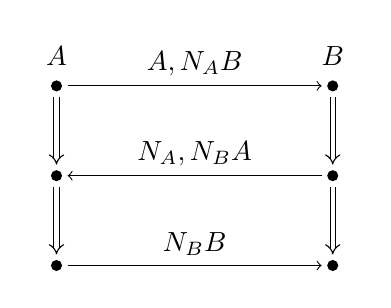
\begin{tikzpicture}[
  implies/.style={double,double equal sign distance,-implies},
  dot/.style={shape=circle,fill=black,minimum size=4pt,
    inner sep=0pt,outer sep=2pt}]

\matrix[matrix of nodes] {
  |[dot,label=above:$A$] (A1)| {} &[3cm] | [dot,label=above:$B$] (B1)| {} \\[1cm]
  |[dot] (A2)| {} & |[dot] (B2)| {}\\[1cm]
  |[dot] (A3)| {} & |[dot] (B3)| {}\\
};
\draw (A1) edge[->] node[above] {$\encrypt{\public{A},N_A}{B}$} (B1)
           edge[implies] (A2);
\draw (B2) edge[->] node[above] {$\encrypt{N_A,N_B}{A}$} (A2)
           edge[implies,implies-] (B1)
           edge[implies] (B3);
\draw (A3) edge[->] node[above] {$\encrypt{N_B}{B}$} (B3)
           edge[implies,implies-] (A2);

\end{tikzpicture}

\appendix

\section{Glossary}

\begin{itemize}
  \squash
\item $\nil$ - null process
\item $\hash{M}$ - hash of $M$
\item $\public{K}$ - public half of asymmetric key $K$
\item $\private{K}$ - private half of asymmetric key $K$
\item $\crypt{M}{K}$ - encrypt $M$ with symmetric key $K$
\item $\encrypt{M}{K}$ - encrypt $M$ with the public key from $K$
\item $\decrypt{M}{K}$ - decrypt $M$ with the public key from $K$
\item $\sign{M}{K}$ - sign $M$ with the private key from $K$
\item $\design{M}{K}$ - check signature on $M$ with the public key from $K$
\item $(\bind{x})P$ - new variable $x$ defined in scope of $P$
\item $\snd{c}{M}$ - send $M$ on channel $c$
\item $\rcv{c}{M}$ - receive $M$ on channel $c$
\item $\rep{P}$ - infinite replication of $P$
\item $P\alt Q$ - $P$ or $Q$
\item $P\cmp Q$ - $P$ in parallel with $Q$
\item $\ccase{\crypt{M}{k}}{x}{P}$ - attempt to decrypt $\crypt{M}{k}$ and
  bind to $x$ in $P$ if successful.  Stuck if unsuccessful
\item $\ccase{\decrypt{M}{k}}{x}{P}$ - attempt to decrypt $\encrypt{M}{k}$ and
  bind to $x$ in $P$ if successful.  Stuck if unsuccessful
\item $\ccase{\design{M}{k}}{x}{P}$ - attempt to check signature $\sign{M}{k}$ and
  bind to $x$ in $P$ if successful.  Stuck if unsuccessful
\item $\icase{x}{y}\arm{0}{P}\arm{suc(x)}{Q}$ - case splitting over integers.
  $x$ is bound in $Q$.
\item $\llet{(x,y)}{M}{y} $ - match $M$ to $(x,y)$ binding $x$ and $y$
  to pair elements in $M$
\item $A\defs B$ - define an equivalence
\item $\sndmsg{A}{B}{M}{c}$ - $A$ sends $B$ message $M$ on channel $c$
\end{itemize}

\begin{align*}
  \label{eq:1}
  A \defs & (\bind{c})\;\snd{c}{M}.\nil \cmp \\
    & \rcv{c}{M}.A
\end{align*}

%%\nocite{}

\bibliography{semantics}

\end{document}
